%
%  Chapter:  2 - Nuclear Models for High Spin Phenomena
%  Modified: 2/16/2015
%  Author:   James Till Matta
%
%%%%%%%%%%%%%%%%%%%%%%%%%%%%%%%%%%%%%%%%%%%%%%%%%%%%%%%%%%

\chapter{NUCLEAR MODELS FOR HIGH SPIN PHENOMENA}
\label{chp:models}

\section{Introduction}
\label{sec:models-into}
The atomic nucleus, discovered in $1911$ by Ernest Rutherford \cite{rutherfordNuclearModel}, is a tiny point of matter at the heart of an atom. The nucleus is approximately $1-10fm$ across, contains more than $99.94\%$ of an atom's mass and is composed of protons and neutrons. Additionally, the nucleus has a powerful short range force that overcomes the Coulomb repulsion to produce a bound system. This force's range is quite limited, perhaps nearest neighbors only as can be seen in the saturation of binding energy per nucleon around $A\sim60$ at a value close to $8.5$MeV.

\begin{figure}[h!]
\centerline{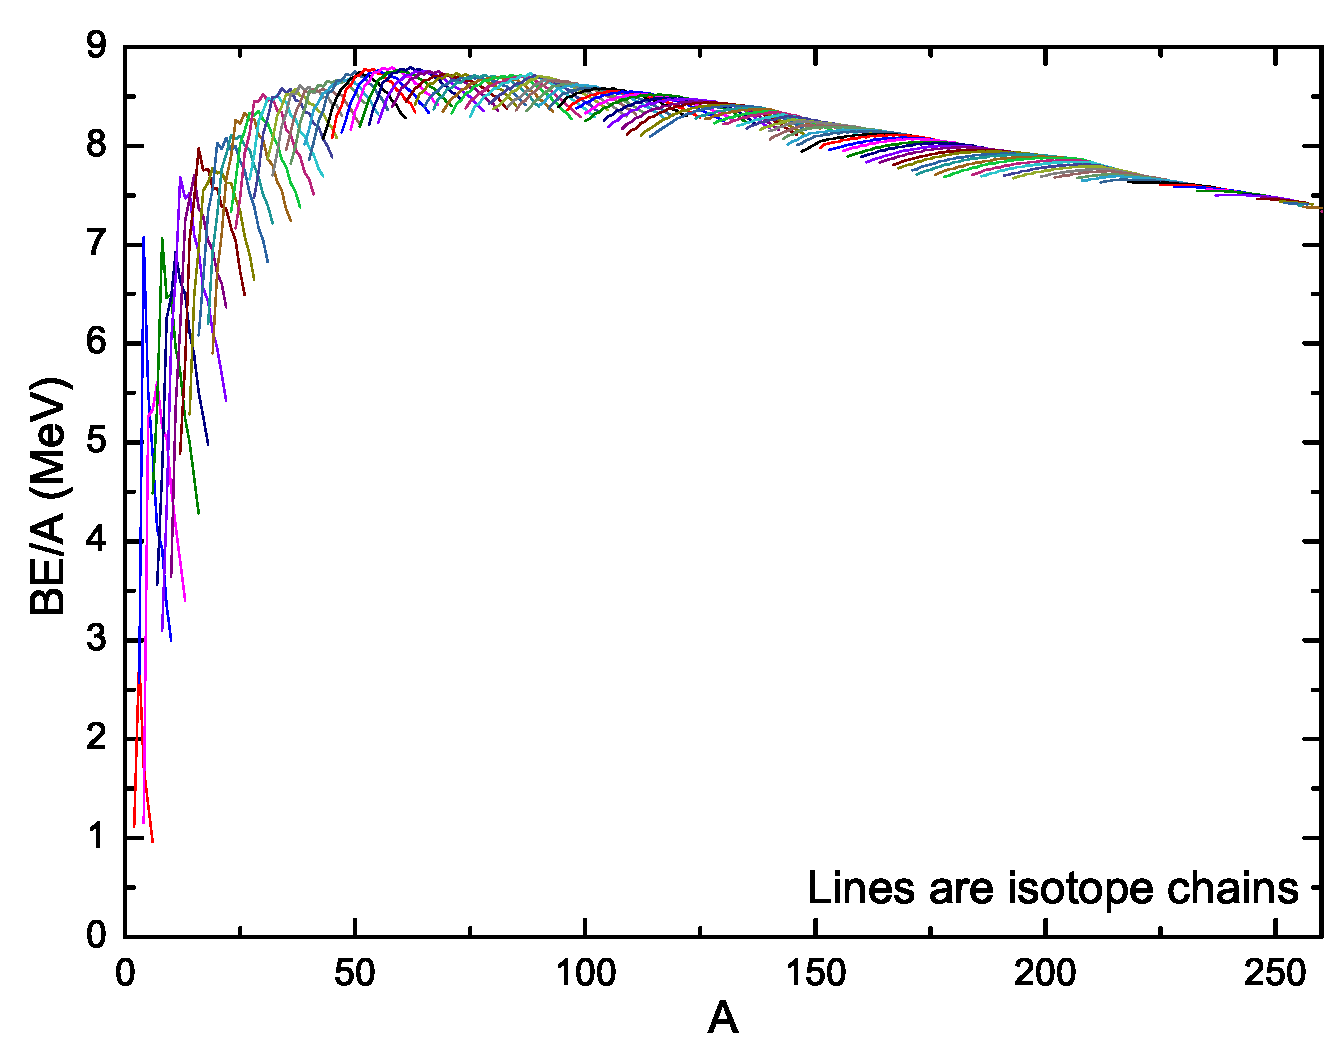
\includegraphics[width=\textwidth]{./img/c2/binding_plot.eps}}
	\caption{Binding energies per nucleon plotted versus mass number. Values calculated from: Ref.\cite{AME20031,AME20032}\label{fig:chp2-binding}}
\end{figure}

Examination of the two proton and two neutron separation energies (Fig \ref{fig:chp2-masses}) shows several distinct discontinuities at specific numbers of protons or neutrons. Further examination of the energies of the first $2^+$ (Fig \ref{fig:chp2-two-plus-energies}) states show peaks at the same numbers. These ``Magic Numbers'' occur at numbers of protons and neutrons where there is a dramatic drop off in the nucleus' stability with the addition of another nucleon. Further evidence for magic numbers of protons and neutrons can be found in the near zero quadrupole moments of nuclei located at these magic numbers, substantially decreased neutron absorption cross-sections at neutron magic numbers, and enhanced abundance for nuclides where N and Z are magic numbers. The magic numbers are $2$, $8$, $20$, $28$, $50$, $82$, and $126$, with $40$ and $64$ also weakly magic over certain ranges of N and Z.

\begin{figure}[h!]
\centerline{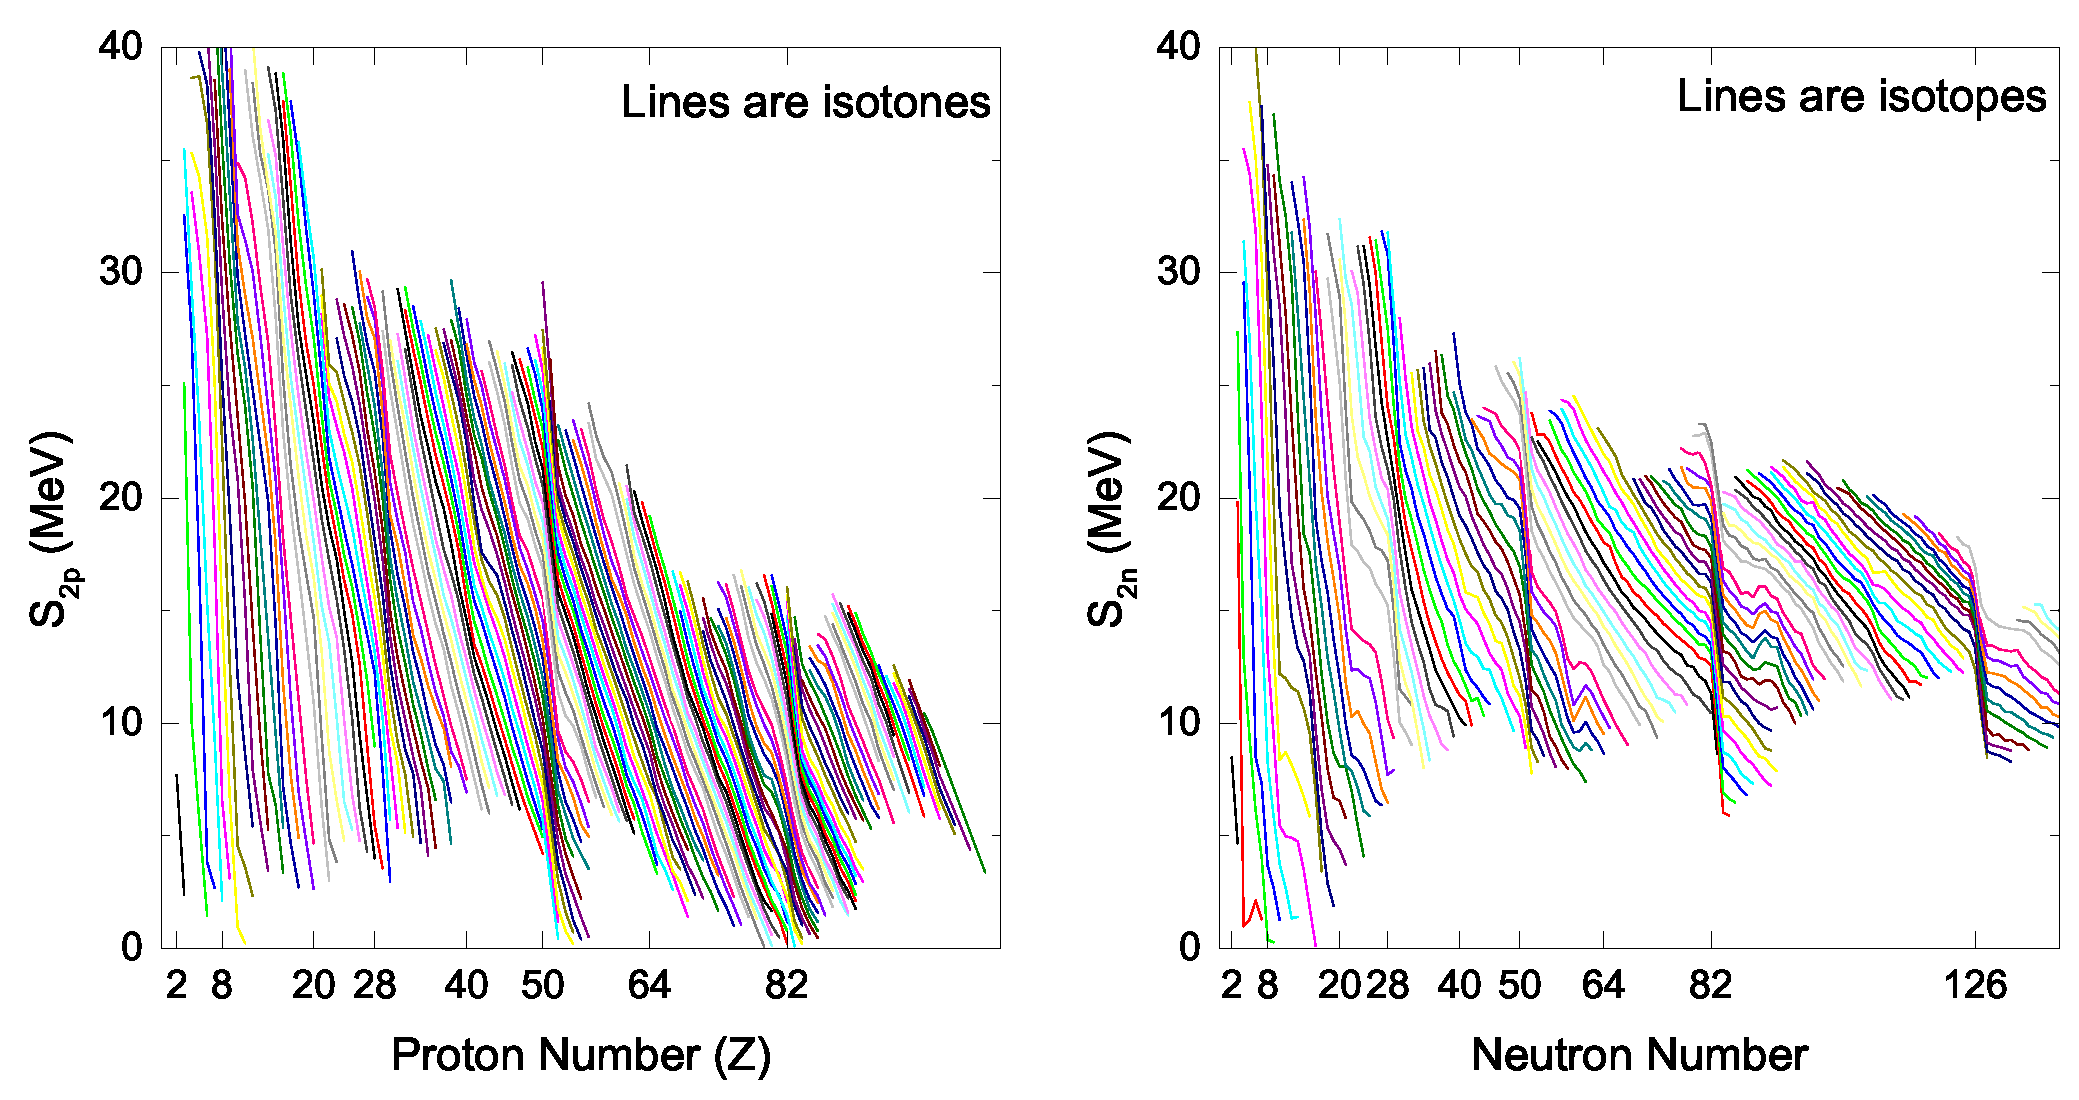
\includegraphics[width=\textwidth]{./img/c2/2nuc_sep_en.eps}}
	\caption{Left: Two proton separation energies plotted versus proton number. Each line is a set of isotones. Right: Two neutron separation energies plotted versus neutron number. Each line is a set of isotopes. Values calculated from: Ref.\cite{AME20031,AME20032}\label{fig:chp2-masses}}
\end{figure}

\begin{figure}[h!]
\centerline{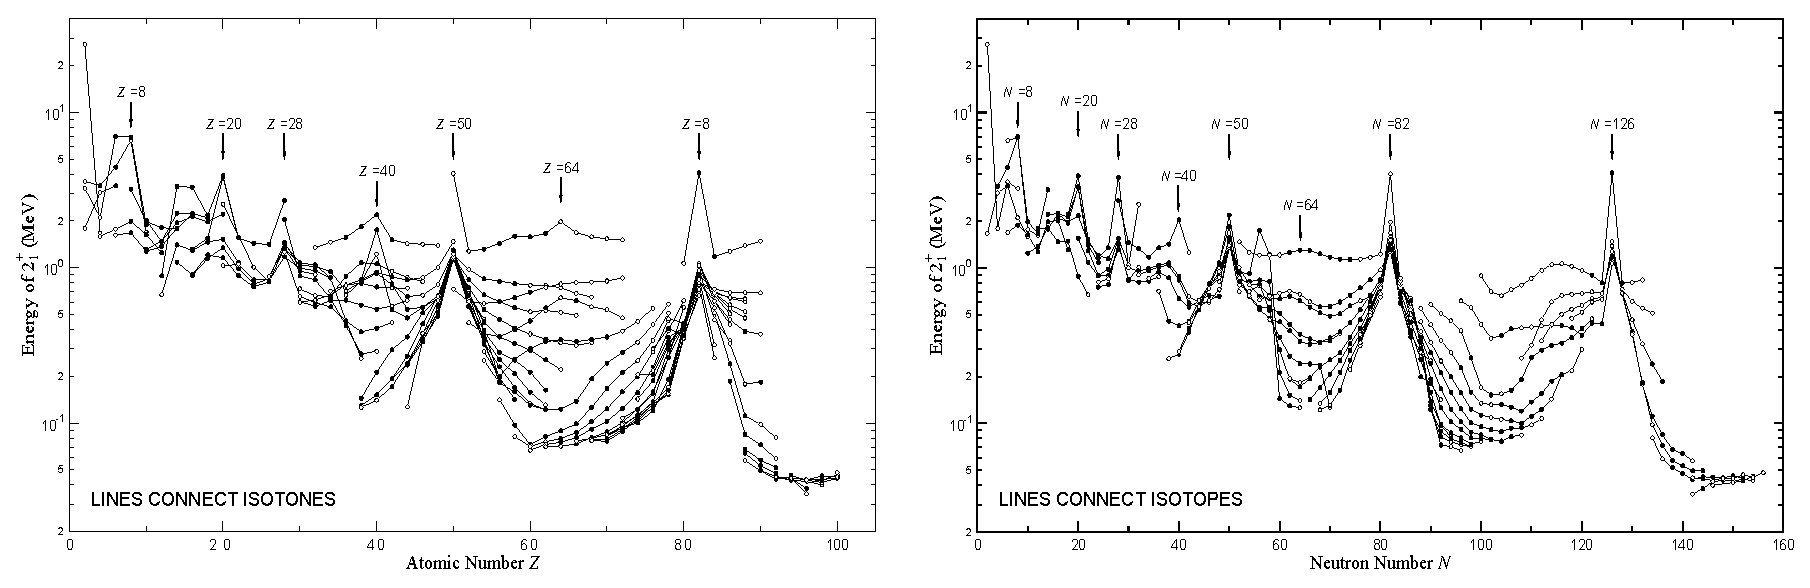
\includegraphics[width=\textwidth]{./img/c2/2_plus_en.eps}}
	\caption{Left: First excited $2^+$ energies of nuclei with even Z and N, plotted versus proton number. Each line is a set of isotones. Right: First excited $2^+$ energies of nuclei with even Z and N, plotted versus neutron number. Each line is a set of isotopes. Figures adapted from: Ref.\cite{RamanTwoPlus}\label{fig:chp2-two-plus-energies}}
\end{figure}

Analogy to atomic theory reveals these magic numbers are major shell closures. This leads to the conclusion that the nucleus has shell structure, leading to the shell model of the nucleus. These numbers can be derived from the calculation of a single particle in a mean field potential. A caveat on these magic numbers is that, far from stability, quenching of the know shell gaps and the opening of new shell gaps has been observed \cite{changingShells}.

Contrariwise, in seeming contradiction to the preceding analogy to atomic theory, the nucleus also exhibits collective excitations such as rotation and vibration which are described later in the chapter. The crucial difference between an atomic system and the nuclear system lies in its occupation of the shells with two types of particles, protons and neutrons. With this, certain shell occupation can lead to the ``single particle behavior'' exhibited around closed shells, while a different occupation can yield collective phenomena.

\section{The Shell Model}
\label{sec:models-shell-model}
The nuclear shell model, in its simplest incarnation, seeks to explain the shell structure observed in nuclei by describing them and independent particles in a mean field potential produced by the other nucleons. While the short range nature of the nuclear force might lead one to use a square well potential or similar as the mean field, the Simple Harmonic Oscillator (SHO) potential is a reasonable first order approximation (seen in Figure \ref{fig:chp2-SHOPot}), which happens to be much simpler to solve. Placing a single particle in the SHO potential gives the first few magic numbers observed; however, to reproduce all the magic numbers it is necessary to add a centrifugal $\vec{l}^2$ potential and a strong spin-orbit ($\vec{l}\cdot\vec{s}$ potential. The Hamiltonian for such a potential is as follows:
\begin{equation}
\label{eqn:chp2-sm-sho-hamil}
\mathbf{\mathit{H}} = \frac{-\hbar^2}{2m}\nabla^2 + \frac{1}{2}m(\omega r)^2 + \beta \uvec{l}^2 + \alpha \uvec{l}\cdot{}\uvec{s}
\end{equation}
The progression of shell gaps from $SHO$ to $SHO + \vec{l}^2$ to $SHO + \uvec{l}^2 + \uvec{l}\cdot\uvec{s}$ is shown in Figure \ref{fig:chp2-shell-model}.

\begin{figure}
\label{fig:chp2-SHOPot}
\centerline{\includegraphics[height=0.25\textheight]{./img/c2/sho_approx.png}}
	\caption{Schematic of a square well, SHO potential, and a realistic Woods-Saxon potential. Figure adapted from: Ref.\cite{casten}}
\end{figure}

\begin{figure}
\label{fig:chp2-shell-model}
\centerline{\includegraphics[height=0.45\textheight]{./img/c2/shell_model.png}}
	\caption{Spectrum of a single nucleon in an SHO potential, SHO + centrifugal potential, and, finally, SHO + centrifugal + spin-orbit. Figure adapted from: Ref.\cite{casten}}
\end{figure}

In more realistic shell model calculations the SHO potential is discarded and a Woods-Saxon potential is adopted. Here the Hamiltonian becomes:
\begin{equation}
\label{eqn:chp2-sm-ws-hamil}
\mathbf{\mathit{H}} = \frac{-\hbar^2}{2m}\nabla^2 + \frac{V}{1+e^{(r-R)/a}} - \alpha(r)\uvec{l}\cdot\uvec{s}
\end{equation}
where $R=r_0A^{1/3}$, $r_0\sim1.2$fm, $a\sim0.5$fm, and $V\sim50$MeV. In addition to the Woods-Saxon component, a spin orbit term is again necessary to reproduce the observed shell gaps. The central flatness of the Woods-Saxon potential mimics the saturation of the nuclear force better than an SHO potential. This increased realism comes at the cost of increase difficulty in calculations and the loss of quantum numbers, in this model the only good quantum numbers are $J=\mathit{l}+\mathit{s}$ and $\pi = (-1)^\mathit{l}$.

Until this point, the nucleons were considered as independent particles with in a mean field which was the average potential produced by the other particles. This description, while powerful, is not accurate, especially for nuclei away from the closed shells. The missing piece is the interactions between nuclei that are not accounted for in the mean field, often called ``residual interactions''. Residual interactions must be accounted for to produce an accurate description of the nucleus.

\section{The Deformed Shell Model}
\label{ssec:models-shell-model-def-sm}
\subsection{Parameterization of Deformation}
In the standard shell model the potentials are spherically symmetric, depending only on the radius. While this is a successful approach near the shell gaps where nuclei are spherical, or nearly spherical, this breaks down in the deformed regions further from shell closures. In such nuclei, the effective long-range forces experienced by the valence nucleons can lead to deformation as the valence nucleons are arranged into deformed shells with lower energy levels. When the nuclear shape is deformed the surface of the nucleus is described with a parametric function defining the radius as follows:
\begin{equation}
\label{eqn:surface-full-expansion}
R(\theta, \phi) = R_{o}\left \lgroup 1 + \sum_{\lambda = 2}^{\infty}\sum_{\mu = -\lambda}^{\lambda}\alpha_{\lambda \mu} Y_{\lambda \mu}(\theta, \phi)\right \rgroup
\end{equation} 
Here $R_0$ is the radius of a sphere with the same volume as the deformed nucleus, $Y_{\lambda \mu}(\theta, \phi)$ are the spherical harmonic functions, and $\alpha_{\lambda \mu}$ are the coefficients of the expansion. The expansion starts at $\lambda = 2$ because the $\lambda = 1$ corresponds to the translation of the center of mass, a term easily eliminated by requiring the nuclear center of mass to coincide with the coordinate's origin. The first of the non-trivial terms, $\lambda = 2$, corresponds to the components of quadrupole deformation, $\lambda = 3$ gives octupole deformation, $\lambda = 4$ gives hexadecapole deformation, so on and so forth. As $\lambda = 2$ is the most important component in this work, only quadrupole deformation terms will be considered from this point on.

The quadrupole shapes cover oblate spheres (two semi-major axes, like a pumpkin), prolate spheres (two semi-minor axes, like an American football), and triaxial shapes (all three axes are different lengths, like a potato). To preserve spheroidal symmetry $R(\theta,\phi) = R(\pi - \theta,-\phi)$ the five quadrupole shape parameters are reduced to two independent parameters $a_{2 0}$ and $a_{2 2}$, with the conditions: $a_{2 -2}=a_{2 2}$ and $a_{2 1}=a_{2 -1}=0$. Further, it is common to parameterize the remaining expansion coefficients using the Hiller-Wheeler variables, $\beta$ and $\gamma$, as follows \cite{wongBook}:
\begin{align}
\label{eqn:chp2-hiller-wheeler}
a_{2 0} = \beta Cos(\gamma)  & &  a_{2 2} = a_{2 -2} = \frac{1}{\sqrt{2}}\beta Sin(\gamma)
\end{align}
Expanding the spherical harmonics as:
\begin{align}
\label{eqn:spherical-harmonics}
Y_{2 0}(\theta, \phi) &= \frac{1}{4} \sqrt{\frac{5}{\pi }} \left(-1+3 Cos(\theta )^2\right)\\
Y_{2 2}(\theta, \phi) &= \frac{1}{4} e^{2 i \phi } \sqrt{\frac{15}{2 \pi }} Sin(\theta)^2\\
Y_{2 -2}(\theta, \phi) &= \frac{1}{4} e^{-2 i \phi } \sqrt{\frac{15}{2 \pi }} Sin(\theta)^2
\end{align} 
and inserting all this into Equation \ref{eqn:surface-full-expansion} yields:
\begin{equation}
\label{eqn:quadrupole-surface}
R(\theta, \phi) = R_{o}\left(1+\sqrt{\frac{5}{16 \pi }}\beta  \left(Cos(\gamma ) \left(3 Cos(\theta )^2-1\right)+\sqrt{3} Sin(\gamma ) Sin(\theta )^2Cos(2 \phi ]\right)\right)
\end{equation} 
The Hiller-Wheeler variables have some redundancy, for $\beta>0$ the nucleus is prolate for $\gamma=0^{\circ},120^{\circ},240^{\circ}$ and oblate for $\gamma=180^{\circ},300^{\circ},60^{\circ}$. However, for $\gamma=0^{\circ}$ and $\gamma=180^{\circ}$ the symmetry axis is the $\uvec{z}$-axis of the intrinsic frame, for $\gamma=120^{\circ}$ and $\gamma=300^{\circ}$ the symmetry axis is the $\uvec{x}$-axis, and for $\gamma=240^{\circ}$ and $\gamma=60^{\circ}$ the symmetry axis is the $\uvec{y}$-axis. The Lund convention makes use of this redundancy by establishing the following rules \cite{wongBook}:
\begin{enumerate}
\item $\beta\geq0$
\item For rotation about the smallest axis $0^{\circ}\leq\gamma\leq60^{\circ}$
\item For rotation about the longest axis $-120^{\circ}\leq\gamma\leq-60^{\circ}$
\item For rotation about the intermediate axis $-60^{\circ}\leq\gamma\leq0^{\circ}$
\end{enumerate}
A graphical schematic of the Lund convention is found in Figure \ref{fig:chp2-lund}
\begin{figure}
\label{fig:chp2-lund}
\centerline{\includegraphics[height=0.25\textheight]{./img/c2/lundconv.png}}
	\caption{Schematic of the Lund convention. Figure adapted from: Ref. \cite{danielDissertation}.}
\end{figure}
\subsection{The Nilsson Model}
To correct the shell model's deficiencies in treating deformed nuclei, in 1955 S.G. Nilsson introduced a modified version of the shell model in Ref \cite{nilsson}. Often called the Nilsson Model

\begin{figure}
\label{fig:chp2-nillson-protons}
\centerline{\includegraphics[height=0.8\textheight,clip=true,trim=10 100 10 100]{./img/c2/nilsson_proton_diagram.pdf}}
	\caption{Nilsson diagram for protons in the $50\leq Z \leq 82$ region with $\epsilon_4=\epsilon_2/6$. Solid lines represent positive parity orbitals and dashed lines represent negative parity orbitals. Labels follow the $\Omega$[N $n_z$ $\Lambda$] convention. Figure adapted from: Ref. \cite{nilssonDiagrams}.}
\end{figure}

\begin{figure}
\label{fig:chp2-nillson-neutrons}
\centerline{\includegraphics[height=0.8\textheight,clip=true,trim=10 100 10 100]{./img/c2/nilsson_neutron_diagram.pdf}}
	\caption{Nilsson diagram for neutrons in the $50\leq N \leq 82$ region with $\epsilon_4=\epsilon_2/6$. Solid lines represent positive parity orbitals and dashed lines represent negative parity orbitals. Labels follow the $\Omega$[N $n_z$ $\Lambda$] convention. Figure adapted from: Ref. \cite{nilssonDiagrams}.}
\end{figure}

\section{Rigid Rotor Model}
\label{sec:models-rigid-rotor}

\section{Tilted Axis Cranking}
\label{sec:models-tac}

\section{Wobbling Vibrations in Nuclei}
\label{sec:models-wobbling}
\subsection{Quasiparticle Triaxial Rotor (QTR)}
\label{sec:models-qtr}
\subsection{Signatures of Wobbling}
\label{sec:models-sig}
